\documentclass[10pt]{article}
\usepackage[scaled=0.92]{helvet}
\usepackage{calc}
\usepackage{multicol}
\usepackage{ifthen}
\usepackage[a4paper,margin=2mm,landscape]{geometry}
\usepackage{amsmath,amsthm,amsfonts,amssymb}
\usepackage{color,graphicx,overpic}
\usepackage{hyperref}
\usepackage{newtxtext} 
\usepackage{enumitem}
\usepackage{amssymb}
\usepackage[table]{xcolor}
\usepackage{vwcol}
\usepackage{tikz}
\usetikzlibrary{arrows.meta}
\usetikzlibrary{calc}
\usepackage{mathtools}
\usepackage{nicematrix}
% for relations
\usepackage{cancel}
\usepackage{ mathrsfs }
\usepackage{minted}
\usemintedstyle{tango}
\definecolor{newblue}{HTML}{ADD8E6}
\colorlet{lightblue}{newblue!45}
\graphicspath{ {./images/} }
\setlist{nosep}

\pdfinfo{
  /Title (CS2030S.pdf)
  /Creator (TeX)
  /Producer (pdfTeX 1.40.0)
  /Author (Ivan Chiew)
  /Subject (CS2030S)
  /Keywords (CS2030S, nus,cheatsheet,pdf)}

% Turn off header and footer
\pagestyle{empty}

\newenvironment{tightcenter}{%
  \setlength\topsep{0pt}
  \setlength\parskip{0pt}
  \begin{center}
}{%
  \end{center}
}

% redefine section commands to use less space
\makeatletter
\renewcommand{\section}{\@startsection{section}{1}{0mm}%
                                {-0.5ex plus -.3ex minus -.2ex}%
                                {0.3ex plus .2ex}%x
                                {\normalfont\large\bfseries}}
\renewcommand{\subsection}{\@startsection{subsection}{2}{0mm}%
                                {-0.5ex plus -.3ex minus -.2ex}%
                                {0.3ex plus .2ex}%
                                {\normalfont\normalsize\bfseries}}
\renewcommand{\subsubsection}{\@startsection{subsubsection}{3}{0mm}%
                                {-0.5ex plus -.3ex minus -.2ex}%
                                {0.5ex plus .2ex}%
                                {\normalfont\small\bfseries}}%
\renewcommand{\familydefault}{\sfdefault}
\renewcommand\rmdefault{\sfdefault}
% makes nested numbering (e.g. 1.1.1, 1.1.2, etc)
\renewcommand{\labelenumii}{\theenumii}
\renewcommand{\theenumii}{\theenumi.\arabic{enumii}.}
\renewcommand\labelitemii{•}
%  for logical not operator
\renewcommand{\lnot}{\mathord{\sim}}
\renewcommand{\bf}[1]{\textbf{#1}}
\newcommand{\abs}[1]{\vert #1 \vert}
\newcommand{\Mod}[1]{\ \mathrm{mod}\ #1}

\makeatother
\definecolor{myblue}{cmyk}{1,.72,0,.38}
\everymath\expandafter{\the\everymath \color{myblue}}
% Define BibTeX command
\def\BibTeX{{\rm B\kern-.05em{\sc i\kern-.025em b}\kern-.08em
    T\kern-.1667em\lower.7ex\hbox{E}\kern-.125emX}}
\let\iff\leftrightarrow
\let\Iff\Leftrightarrow
\let\then\rightarrow
\let\Then\Rightarrow

% Don't print section numbers
\setcounter{secnumdepth}{0}

\setlength{\parindent}{0pt}
\setlength{\parskip}{0pt plus 0.3ex}
%% this changes all items (enumerate and itemize)
\setlength{\leftmargini}{0.5cm}
\setlength{\leftmarginii}{0.5cm}
\setlist[itemize,1]{leftmargin=1.5mm,labelindent=0.5mm,labelsep=0.5mm}
\setlist[itemize,2]{leftmargin=3mm,labelindent=0.5mm,labelsep=0.5mm}

%My Environments
\newtheorem{example}[section]{Example}
% -----------------------------------------------------------------------

\begin{document}
\raggedright
\footnotesize
\begin{multicols}{3}


% multicol parameters
% These lengths are set only within the two main columns
\setlength{\columnseprule}{0.25pt}
\setlength{\premulticols}{1pt}
\setlength{\postmulticols}{1pt}
\setlength{\multicolsep}{1pt}
\setlength{\columnsep}{1.5pt}

\begin{center}
    \fbox{%
        \parbox{0.6\linewidth}{\centering \textcolor{black}{
            {\normalsize\textbf{CS2030S}}
            \\ \small{AY25/26 Sem 1}}
            \\ {\scriptsize \textcolor{myblue}{Programming Methodology II}} 
        }%
    }
\end{center}

\section{Programming Languages}
\textbf{Dynamic vs Static Typing}: Dynamic -- variables can hold values of multiple different unrelated types. Static -- variable types must be declared and cannot be changed.\\
\textbf{Strong vs Weak Typing}: Stronger languages have greater rules in their type system to ensure type safety.

\section{Tombstone Diagram}
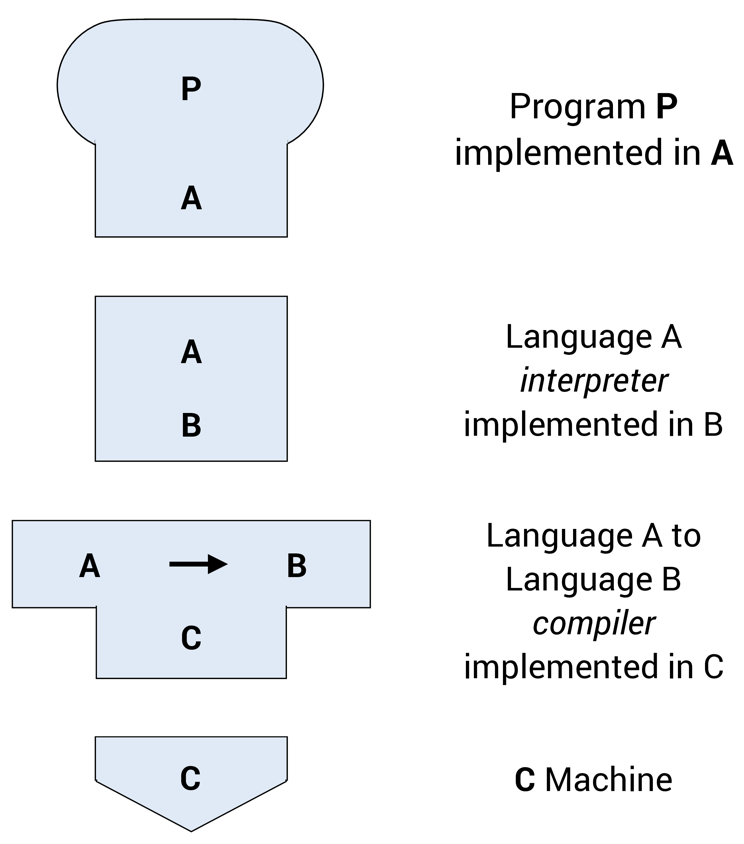
\includegraphics[width=0.55\linewidth]{tombstone.png}

\section{Subtyping}
T is a subtype of S (\texttt{T <: S}) if code written for S can be safely used for T. T has narrower scope, S has wider scope.
\begin{itemize}
  \item \textbf{Widening}: T can be put into S
  \item \textbf{Narrowing}: S can be explicitly typecast into T
  \item \textbf{Reflexive}: T $<:$ T
  \item \textbf{Transitive}: T $<:$ S, S $<:$ U $\Rightarrow$ T $<:$ U
  \item \textbf{Anti-Symmetric}: T $<:$ S, S $<:$ T $\Rightarrow$ S = T
\end{itemize}

\section{Primitive Types}
\begin{itemize}
  \item \textbf{Numeric}: byte $<:$ short $<:$ int $<:$ long $<:$ float $<:$ double
  \item \textbf{Character}: char $<:$ int
  \item \textbf{Boolean}: boolean
  \item \textbf{Void}: void (no value)
\end{itemize}

\section{Reference Types}
Anything not a primitive type (e.g., classes). Stores only a reference to the value. Two reference variables can share the same value -- equality by default compares references. Uninitialized: null value, throws \texttt{NullPointerException}.

\section{01 OOP Fundamentals}
\subsection{Encapsulation}
Bundle data and methods within a single unit (class). Hide internal state.
\begin{minted}[breaklines,breakanywhere,bgcolor=lightblue]{java}
class Circle {
    private double radius;
    
    public Circle(double radius) {
        this.radius = radius;
    }
    
    public double getRadius() { return radius; }
    public double getArea() { 
        return Math.PI * radius * radius; 
    }
}
\end{minted}

\subsection{Immutability}
Object state cannot be modified after creation. Use \texttt{final}.
\begin{minted}[breaklines,breakanywhere,bgcolor=lightblue]{java}
class ImmutablePoint {
    private final double x;
    private final double y;
    
    public ImmutablePoint(double x, double y) {
        this.x = x;
        this.y = y;
    }
    
    public ImmutablePoint move(double dx, double dy) {
        return new ImmutablePoint(x + dx, y + dy);
    }
}
\end{minted}

\subsection{Tell, Don't Ask}
Tell objects what to do; don't ask for their state.
\begin{minted}[breaklines,breakanywhere,bgcolor=lightblue]{java}
// Bad
if (circle.getRadius() > 5) { /* ... */ }

// Good
circle.isLargerThan(5.0)
\end{minted}

\section{Stack and Heap}
\textbf{Stack}: Where all variables are allocated and stored. Contains \textbf{Call Frames}, created when methods are invoked and destroyed when returned.\\
\textbf{Heap}: Where objects are allocated and stored. Whenever \texttt{new} is used, a new object is created on the heap. Objects store: Class Name, Instance Fields and Values, Captured Variables.

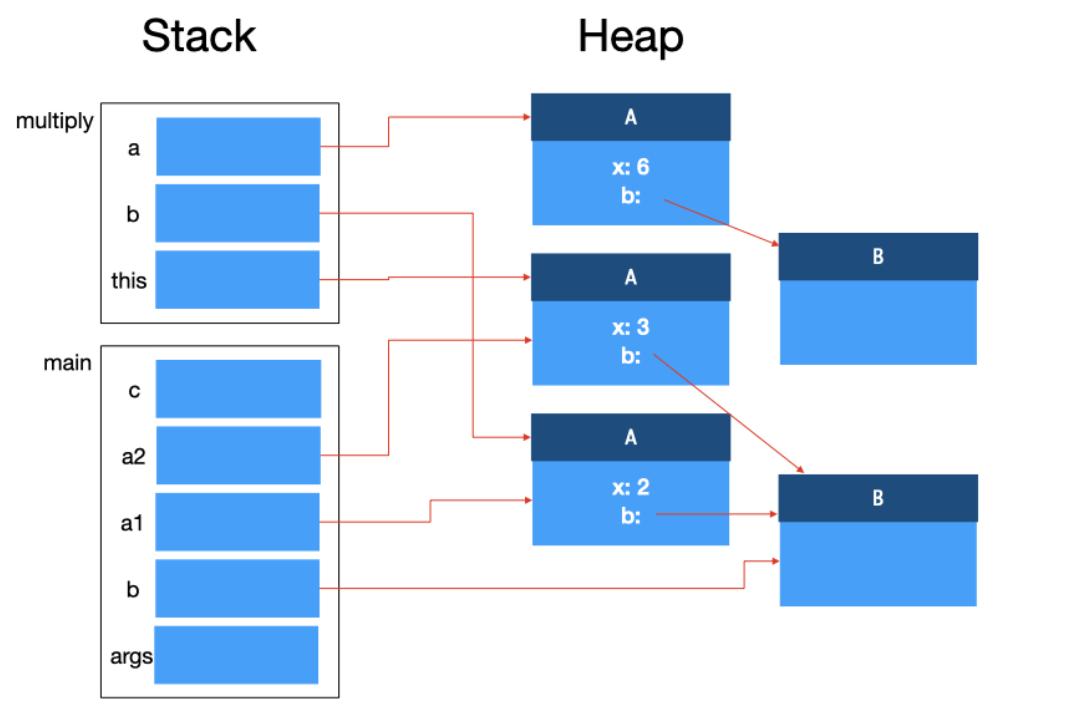
\includegraphics[width=0.85\linewidth]{stacknheap.png}

\section{Class Fields and Methods}
\begin{itemize}
  \item Use \texttt{static} keyword for class-level fields/methods
  \item Fields accessed via \texttt{Class.field} (shared across entire class)
  \item Methods accessed via \texttt{Class.method()}, but \texttt{this} will \textbf{NOT} work
\end{itemize}

\section{02 Inheritance \& Polymorphism}
\subsection{Inheritance}
\begin{minted}[breaklines,breakanywhere,bgcolor=lightblue]{java}
class Shape {
    private String color;
    public Shape(String color) {
        this.color = color;
    }
    double getArea() { return 0; }
}

class Circle extends Shape {
    private double radius;
    
    public Circle(double radius, String color) {
        super(color); // MUST BE FIRST LINE
        this.radius = radius;
    }
    
    @Override
    double getArea() {
        return Math.PI * radius * radius;
    }
}
\end{minted}
\textbf{Overriding}: Use \texttt{@Override}. Must match Method Descriptor (Name, Parameters, Return Type).\\
\textbf{Overloading}: Same name, different Method Signature (Name, Parameter Types).

\subsection{Polymorphism}
Same interface, different implementations.
\begin{minted}[breaklines,breakanywhere,bgcolor=lightblue]{java}
Shape s1 = new Circle(5.0, "red");
Shape s2 = new Rectangle(3.0, 4.0, "blue");

double area1 = s1.getArea(); // Circle's getArea
double area2 = s2.getArea(); // Rectangle's getArea
\end{minted}

\subsection{Abstract Classes}
A general class that should \textbf{NEVER} be instantiated. Abstract arrays can still be defined. Abstract methods have no body. A class with abstract methods must be made abstract.
\begin{minted}[breaklines,breakanywhere,bgcolor=lightblue]{java}
abstract class Shape {
    abstract double getArea();
    abstract double getPerimeter();
    
    // Concrete method
    public void printInfo() {
        System.out.println("Area: " + getArea());
    }
}
\end{minted}

\subsection{Interfaces}
Models requirements of classes. Methods are \texttt{public abstract} by default. A class can implement multiple interfaces (solves Diamond Problem). Can be impure using \texttt{default} keyword.
\begin{minted}[breaklines,breakanywhere,bgcolor=lightblue]{java}
interface Drawable {
    void draw();
    default void info() { /* body */ } // impure
}

class Circle implements Drawable, Comparable<Circle> {
    public void draw() { /* ... */ }
    public int compareTo(Circle other) {
        return Double.compare(this.radius, other.radius);
    }
}
\end{minted}

\subsection{Liskov Substitution Principle (LSP)}
Any property of objects of type T should be true for any object of type S where S $<:$ T. Don't break expectations of the parent class. Can use \texttt{final} to prevent inheritance or modification of methods/fields.
\begin{minted}[breaklines,breakanywhere,bgcolor=lightblue]{java}
void processShape(Shape s) {
    double area = s.getArea(); // works for all
}

processShape(new Circle(5.0));
processShape(new Rectangle(3.0, 4.0));
\end{minted}

\section{Dynamic Binding}
\textbf{CTT (Compile Time Type)}: Declared type of variable.\\
\textbf{RTT (Run Time Type)}: Actual type of object at runtime.
\begin{minted}[breaklines,breakanywhere,bgcolor=lightblue]{java}
Circle c = new ColouredCircle();
// CTT(c) = Circle, RTT(c) = ColouredCircle
\end{minted}
For \texttt{obj.foo(arg)}:\\
\textbf{Compile Time}:
\begin{itemize}
  \item Check CTT(obj); find all accessible \texttt{foo} methods (including supertypes of CTT(obj))
  \item Find most specific method fitting CTT(arg); record method descriptor
\end{itemize}
\textbf{Run Time}:
\begin{itemize}
  \item Retrieve method descriptor; determine RTT(obj)
  \item From RTT(obj), find first fitting method descriptor; recurse upwards until found
\end{itemize}
Does \textbf{not} apply to class (static) methods.

\section{Wrapper Classes}
Java provides wrapper classes for primitive types (e.g., \texttt{Integer}, \texttt{Double}).
\begin{minted}[breaklines,breakanywhere,bgcolor=lightblue]{java}
Integer i = 4;  // auto-boxing (line 1)
int j = i;      // auto-unboxing (line 2)
\end{minted}
\begin{itemize}
  \item \textbf{Auto-boxing}: Automatically put primitive into wrapper class
  \item \textbf{Auto-unboxing}: Automatically get value from wrapper class
  \item 2-step boxing \textbf{NOT} allowed (e.g., \texttt{Double d = 2})
  \item Wrapper classes \textbf{DO NOT} share subtyping with primitives
  \item Performance cost: objects stored on heap; wrapper classes are immutable
\end{itemize}

\section{Type Checking}
\texttt{a = (C) b}: where \texttt{b} has CTT(b) and RTT(b).
\begin{itemize}
  \item Find CTT(b); check if possible for RTT(b) $<:$ C
  \begin{itemize}
    \item CTT(b) $<:$ C: widening cast, allowed at compile time
    \item C $<:$ CTT(b): narrowing, requires runtime check for RTT(b)
    \item C is interface: could be a subclass of B implementing C
  \end{itemize}
  \item \textbf{Impossibility}: B and C are unrelated; C is interface and B is final
  \item Find CTT(a): check C $<:$ CTT(a); add runtime check for RTT(b) $<:$ C
  \item \textbf{Run Time}: Find RTT(b); check if RTT(b) $<:$ C
\end{itemize}

\section{Variance}
\begin{itemize}
  \item \textbf{Covariant}: S $<:$ T implies S[] $<:$ T[] (Java arrays are covariant)
  \item \textbf{Contravariant}: S $<:$ T implies (T) $<:$ (S)
  \item \textbf{Invariant}: None of the above (Java generics are invariant)
\end{itemize}

\section{03 Generics}
\subsection{Generic Class}
\begin{minted}[breaklines,breakanywhere,bgcolor=lightblue]{java}
class Box<T> {
    private T item;
    
    public Box(T item) { this.item = item; }
    public T getItem() { return item; }
    
    public <U> Box<U> map(Transformer<T, U> f) {
        return new Box<>(f.transform(item));
    }
}

Box<String> strBox = new Box<>("hello");
\end{minted}

\subsection{Generic Methods}
\begin{minted}[breaklines,breakanywhere,bgcolor=lightblue]{java}
public static <T extends Comparable<T>> T max(T a, T b) {
    return a.compareTo(b) > 0 ? a : b;
}
\end{minted}

\subsection{Bounded Type Parameters}
\begin{minted}[breaklines,breakanywhere,bgcolor=lightblue]{java}
// Upper bound: T must be Number or subclass
class NumBox<T extends Number> {
    private T value;
    public double getDouble() {
        return value.doubleValue();
    }
}
// Multiple bounds
<T extends Shape & Drawable>
\end{minted}

\subsection{Type Erasure}
After type checking, Java performs type erasure for backwards compatibility. Generic types replaced by upper bound (default Object). When a Generic is instantiated, a typecast is added.
\begin{minted}[breaklines,breakanywhere,bgcolor=lightblue]{java}
// Before erasure
Int i = new Pair<Str,Int>("a", 4).sec();
// After erasure
Int i = (Int) new Pair("a", 4).sec();
\end{minted}
Cannot use: \texttt{new T()}, \texttt{new T[]}, \texttt{T.class}

\subsection{Generic Array Problems}
Due to type erasure, cannot tell if putting Generics into an array will cause errors. Generic array declaration is ok, but instantiation with \texttt{new} is not.
\begin{minted}[breaklines,breakanywhere,bgcolor=lightblue]{java}
// Problem: becomes Pr[] after erasure
Pr<Str,Int>[] pArr = new Pr<Str,Int>[2];
Object[] oArr = pArr;
oArr[0] = new Pr<Dbl,Bool>(3.14, true);
// -> ClassCastException
\end{minted}
Arrays are reifiable (full type info at runtime); generics are not, so Java does not allow creating generic arrays with \texttt{new}.

\subsection{Generic Arrays and Warnings}
Since we cannot instantiate generic arrays, typecast instead (arrays are covariant):
\begin{minted}[breaklines,breakanywhere,bgcolor=lightblue]{java}
T[] tmp = (T[]) new Object[sz];
this.arr = tmp;
\end{minted}
Generates unchecked warning. Suppress with \texttt{@SuppressWarnings("unchecked")} only after justifying: array is \texttt{private} so only accessed by the class; array can only be modified by \texttt{Seq::set(int, T)}, which is of type T; the only retrievable objects from array are subtypes of T via \texttt{Seq::get(int)}.

\subsection{Generic Type Rules}
\begin{itemize}
  \item Generic method signature includes type parameters (equal up to renaming)
  \item Type checking uses type argument for class-level type parameters where possible
  \item Method descriptor stored during dynamic binding at CTT is type erased
\end{itemize}

\subsection{Wildcards}
\begin{minted}[breaklines,breakanywhere,bgcolor=lightblue]{java}
// Upper bounded (covariant)
// copyFrom(Seq<? extends T> src): src is subtype of T
void processShapes(List<? extends Shape> shapes) {
    for (Shape s : shapes) { s.getArea(); } // can read
    // shapes.add(new Circle()); // CANNOT add
}

// Lower bounded (contravariant)
// copyTo(Seq<? super T> dest): dest is supertype of T
void addCircles(List<? super Circle> list) {
    list.add(new Circle(5.0)); // can add
    // Circle c = list.get(0); // CANNOT get
}
\end{minted}
\textbf{PECS}: Producer Extends, Consumer Super\\
\texttt{? extends T} for \textbf{reading} (producer); \texttt{? super T} for \textbf{writing} (consumer)\\
\textbf{Unbounded wildcards}: Similar to Object supertype, but object as a generic type parameter does not work as generics are invariant. Used to replace raw types.

\subsection{Type Inference}
Use empty diamond \texttt{<>} on RHS to instantiate generic types. 3-step method:
\begin{enumerate}
  \item \textbf{Argument Typing}: Type of parameters passed in
  \item \textbf{Target Typing}: Type of variable where return is stored
  \item \textbf{Type Parameter}: Explicitly specified type parameters in the declaration
\end{enumerate}
Java considers types explicitly involved in inequalities, then chooses the most specific type.

\section{Bridge Methods}
Compiler generates bridge methods to preserve polymorphism after type erasure when inheritance and overriding interact with generics.

\textbf{Conditions}: (i) Class is subtype of parameterised type; (ii) Type erasure changes inherited method signature.
\begin{minted}[breaklines,breakanywhere,bgcolor=lightblue]{java}
class Box<T> { void get(T t) {} }
class StringBox extends Box<String> {
  @Override void get(String s) {} // user code
}
// After erasure, compiler generates:
class StringBox extends Box {
  void get(Object s) { this.get((String) s); } // bridge
  void get(String s) {} // user code
}
\end{minted}

\section{06 Exception Handling}
\subsection{Try-Catch-Finally}
\begin{minted}[breaklines,breakanywhere,bgcolor=lightblue]{java}
try {
    int result = riskyOperation();
} catch (SpecificException e) {
    // Handle specific
} catch (Exception e) {
    // Handle general
} finally {
    // Always executed (cleanup)
}
\end{minted}
\textbf{Checked}: Must be caught/declared (Exception)\\
\textbf{Unchecked}: Runtime exceptions (RuntimeException)\\
\texttt{throw} immediately suspends \texttt{try}. \texttt{finally} \textbf{ALWAYS RUNS}.

\subsection{Try-with-Resources}
\begin{minted}[breaklines,breakanywhere,bgcolor=lightblue]{java}
try (FileReader fr = new FileReader("f.txt")) {
    String line = br.readLine();
} // Resources auto-closed
\end{minted}

\end{multicols}

\end{document}
